\documentclass[12pt]{article}

\usepackage[margin=1.0in]{geometry}
\usepackage{tabto}
\usepackage{amsmath}
\usepackage{framed}
\usepackage{graphicx}
\usepackage{listings}
\usepackage{color} %red, green, blue, yellow, cyan, magenta, black, white
\definecolor{mygreen}{RGB}{28,172,0} % color values Red, Green, Blue
\definecolor{mylilas}{RGB}{170,55,241}
\graphicspath{ {./} }

\newcommand*\lstinputpath[1]{\lstset{inputpath=#1}}



\begin{document}

\title{CS / MATH 4334 : Numerical Analysis\\Homework Assignment 6}
\author{Matthew McMillian\\mgm160130@utdallas.edu}
\maketitle

\section*{MatLab Problems}

\lstset{language=Matlab,%
    %basicstyle=\color{red},
    breaklines=true,%
    morekeywords={matlab2tikz},
    morekeywords=[2]{1}, keywordstyle=[2]{\color{black}},
    identifierstyle=\color{black},%
    showstringspaces=false,%without this there will be a symbol in the places where there is a space
    numbers=left,%
    numberstyle={\tiny \color{black}},% size of the numbers
    numbersep=9pt, % this defines how far the numbers are from the text
    emph=[1]{for,end,break},emphstyle=[1]\color{red}, %some words to emphasise
    %emph=[2]{word1,word2}, emphstyle=[2]{style},    
}

\pagebreak

	\begin{enumerate}
	
	\item[] Problem 1 : p1.m \noindent\rule{\textwidth}{1.0pt} \\
	\lstinputlisting{p1.m}	
	
	\pagebreak
	
	\item[] Problem 1 : wtseries.m \noindent\rule{\textwidth}{1.0pt} \\
	\lstinputlisting{wtseries.m}	
	
	\pagebreak	
	
	\item[] Problem 1 : actual.m \noindent\rule{\textwidth}{1.0pt} \\
	\lstinputlisting{actual.m}	
	
	\pagebreak		
	
	$>>$ p1.m
	\begin{framed}

If we increase the number of points by a factor of 10, then our global error decreases by a factor of 10. Thus it has a linear relation, O(h), as we expect.

	\end{framed}
	
	\begin{center}
		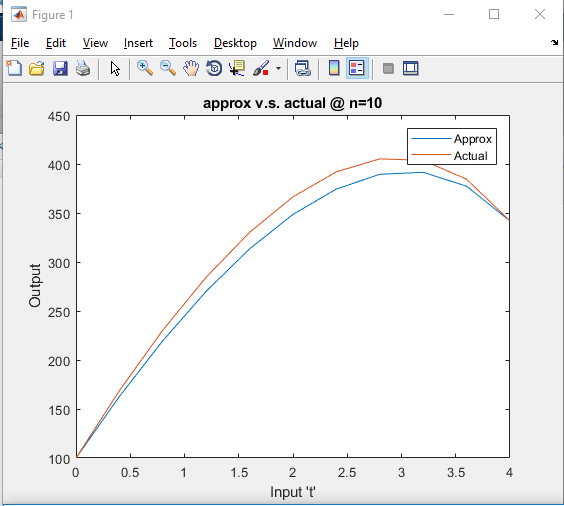
\includegraphics[scale=0.6]{g1}
	\end{center} 
	\begin{center}
		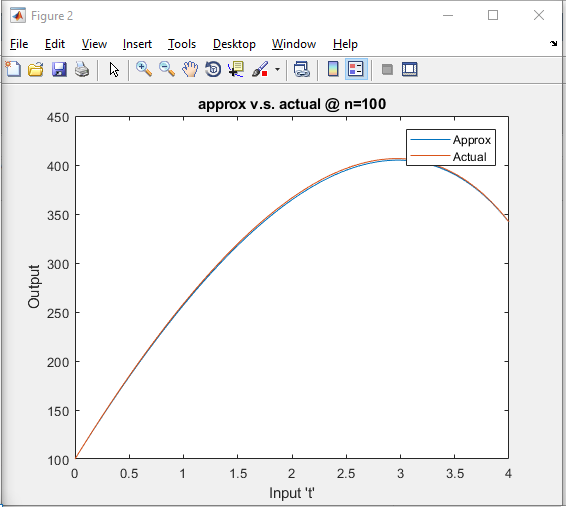
\includegraphics[scale=0.6]{g2}
	\end{center} 
	\begin{center}
		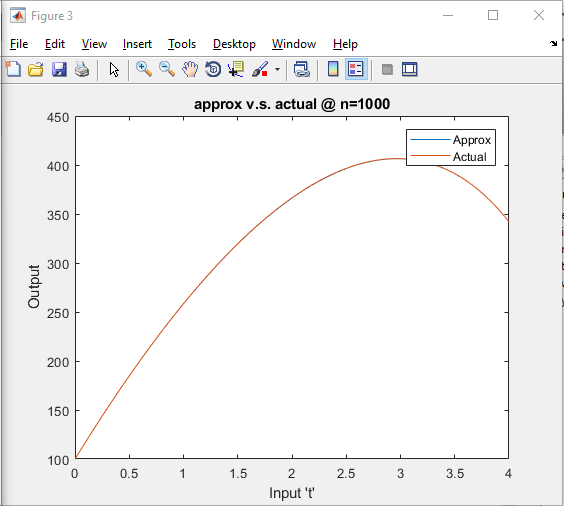
\includegraphics[scale=0.6]{g3}
	\end{center} 
	\begin{center}
		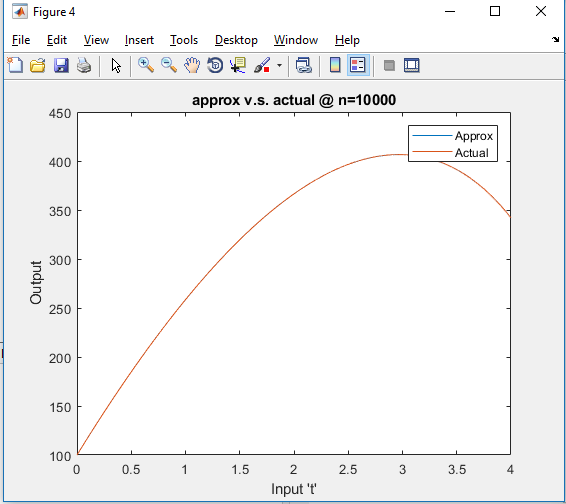
\includegraphics[scale=0.6]{g4}
	\end{center} 
	\begin{center}
		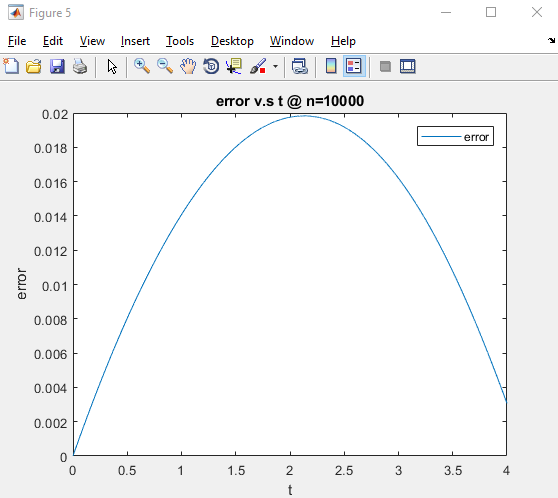
\includegraphics[scale=0.8]{p5}
	\end{center} 
	
	\end{enumerate}
	
	
	
\end{document}